\subsection{Kubernetes Installation}
The Kubernetes master installation is well documented and did not pose any troubles. For completion of this thesis I will briefly mention the additional components installed on the master. Kubernetes has no default networking implementation, thus I installed Flannel\cite{coreosFlannel:online}, one of the simplest and most widely used networking fabrics specifically designed for Kubernetes. It runs a small binary called \textit{flanneld} on each node and provides networking between nodes and pods\footnote{The specifics of Flannels networking are outside this thesis scope, for more information see \url{https://blog.laputa.io/kubernetes-flannel-networking-6a1cb1f8ec7c}}. For administrative purposes I also installed the Kubernetes Dashboard.

The Raspberry Pi Foundation recently released an update to Raspbian (the RPi OS) called buster, which does dropped support of the aufs-dkms kernel modules, which are dependencies of kubeadm and containerd. The online community advised in forums to avoid the dependency but if possible switch back to the older version of Raspbian called stretch. Out of time concerns, I switched back to the old version. 

I switched the official Kubernetes kubelet with the kubelet binary from Ranchers K3s called Hyperkube. \Cref{fig:kubeBinaries} shows the size of the binary files of three most important components of Kubernetes, kubeadm, kubelet and kubectl.
\begin{figure}[h!]
    \centering
    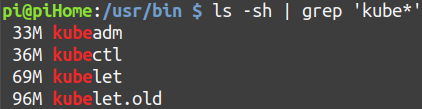
\includegraphics[scale=0.5]{figures/kubeBinariesSize.png}
    \vspace*{-0.3cm}
    \mycaption[The Sizes of the Kubernetes Binaries.]{\\ Note, \textit{kubelet} is the K3s hyperkube binary and \textit{kubelet.old} is the official kubelet bianry.}
    \label{fig:kubeBinaries}
\end{figure}
In total the official binaries are 165 megabyte large and the kubelet (\textit{kubelet.old} file) takes almost half the space. Using the K3s build of kubelet (\textit{kubelet} file) brings the total amount to 138 megabyte saving almost 20\% of space in addition to its other benefits discussed in \cref{sec:Kubernetes} \nameref{sec:Kubernetes}. The full installation procedure can be found in the repository of this thesis for replication and validation.

Finally, the effects on the system resources are two folds, the native applications and the running containers. The Raspberry Pi has 926MB total memory and a 1.4 GHz quad-core CPU. Firstly, \cref{fig:kubernetesResourceConsumption} shows the resource usage of the native applications
\begin{figure}[h!]
    \centering
    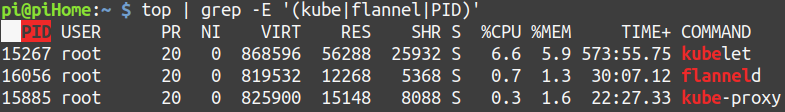
\includegraphics[scale=0.5]{figures/kubernetesResourceConsumption.png}
    \vspace*{-0.3cm}
    \caption[The Resource Usage of native Kubernetes Components.]{Using the K3s hyperkube binary.}
    \label{fig:kubernetesResourceConsumption}
\end{figure}
The kubelet process uses 6.6\% of the CPU and 5.9\% of the memory. While the memory usage is consistent, the CPU usage varies a lot and can reach peaks of 16\%. Using the command
\begin{displayquote}
\textit{top | egrep --line-buffered '(kubelet|PID)' > /home/pi/kubeletHyper.txt }
\end{displayquote}
the cpu usage was tracked over 38 minutes with an average of 3.16 data points per second and a total of 7235 data points\footnote{The entire statistics can be found in the project files together with the source code.}. The average CPU usage in the time period was 10.3\%, the memory usage was constant.

Flanneld and kube-proxy both use less than 1\% CPU and 1.3\% and 1.6\% of memory, respectively. It is important to note that the container runtime is not included in that statistics. The resource usage of the Kubernetes relevant containers is shown in \cref{fig:kubernetesResourceConsumptionCut}\footnote{The figure is cut to fit the page. The full figure can be seen the appendix.}.
\begin{figure}[h!]
    \centering
    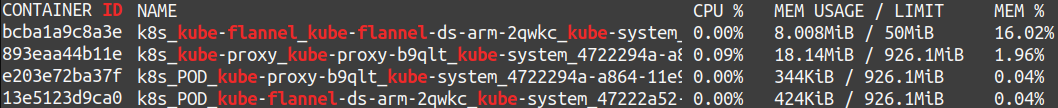
\includegraphics[scale=1.6]{figures/kubeContainerResourceUsageCut.png}
    \vspace*{-0.3cm}
    \caption[The Resource Usage of Kubernetes Containers.]{\\The command used is: \textit{docker stats | grep -E '(ID|kube|flannel)'}.}
    \label{fig:kubernetesResourceConsumptionCut}
\end{figure}
Flannel and kube-proxy consume 0.86\% and 1.96\% of the memory, respectively\footnote{flannel's limit is 50MB, hence the 16.02\% in the figure.}. The CPU usage of all containers is negligible at below 1\%. Adding up the numbers, after the installation Kubernetes uses 11.4\% of the CPU and 11.7\% of the total memory. This translates to 0.46GHz CPU usage, see \cref{eq:cpuTotal}, and 108.35MB memory usage, see \cref{eq:ramTotal}.
\begin{equation} \label{eq:cpuTotal}
    1.4GHz * 4 \; \textrm{(cores)} * 0.114 = 0.638GHz  \quad \textrm{(CPU usage)}
  \end{equation}
  \begin{equation} \label{eq:ramTotal}
    926.1MB * 0.117 = 108.354MB  \quad \textrm{(RAM usage)}
  \end{equation}
The memory consumption is especially concerning as swap needs to be disabled for Kubernetes to install. Swap is a partion in Linux used for paging. If disabled, memory can not be written to disk anymore which can lead to a memory overflow.